%-------------------------------------------------------------------------------
% Preamble
%-------------------------------------------------------------------------------

\documentclass{ametsoc}
\journal{jcli}

%Citations should be of the form ``author year''  not ``author, year''
\bibpunct{(}{)}{;}{a}{}{,}

%Packages
\usepackage{
	siunitx, % units
	cleveref,% cross-references
	physics, % better physics notation
	url, % for URLs
	amsmath, % for math
	array, % for fixed-width tables
	booktabs, % for nice tables
	nth, % for \nth{90}
}
\newcolumntype{L}[1]{>{\raggedright\let\newline\\\arraybackslash\hspace{0pt}}m{#1}}
\graphicspath{{../../figs/}{./}}

\usepackage[acronym]{glossaries}
\makeglossaries
\newacronym{wt}{WT}{weather type}
\newacronym{sallj}{SALLJ}{South American low-level jet}
\newacronym{enso}{ENSO}{El Ni\~{n}o-Southern Oscillation}
\newacronym{mjo}{MJO}{Madden-Julian Oscillation}
\newacronym{sacz}{SACZ}{South Atlantic Convergence Zone}
\newacronym{iri}{IRI}{International Research Institute for Climate and Society}
\newacronym{ecmwf}{ECMWF}{European Centre for Medium-Range Weather Forecasts}
\newacronym{s2s}{S2S}{sub-seasonal to seasonal}
\newacronym{eof}{EOF}{empirical orthogonal function}
\newacronym{mos}{MOS}{model output statistics}
\newacronym{xlr}{XLR}{homoscedastic extended logistic regression}
\newacronym{hxlr}{HXLR}{heteroscedastic extended logistic regression}
\newacronym{pcr}{PCR}{princiap components regression}
\newacronym{cca}{CCA}{canonical correlation analysis}
\newacronym{sst}{SST}{sea surface temperature}

%-------------------------------------------------------------------------------
% Title and Authors
%-------------------------------------------------------------------------------

\title{Heavy rainfall in Paraguay during the 2015-2016 austral summer: causes and sub-seasonal-to-seasonal predictive skill}
\authors{James Doss-Gollin\correspondingauthor{James Doss-Gollin. Columbia Water Center. Dept. of Earth and Environmental Engineering, Columbia University, 500 W. 120th St., New York, NY. USA.}}
\affiliation{Columbia Water Center. Dept. of Earth and Environmental Engineering, Columbia University, 500 W. 120th St., New York, NY. USA \\ Columbia Water Center, Columbia University, 500 W. 120th St., New York, NY. USA}
\email{james.doss-gollin@columbia.edu}
\extraauthor{\'Angel G. Mu\~noz}
\extraaffil{Atmospheric and Oceanic Sciences (AOS). Princeton University. Princeton, NJ 08540-6649. USA  \\
	International Research Institute for Climate and Society (IRI). The Earth Institute. Columbia University. Palisades, NY. 10964-1000. USA}
\extraauthor{Simon J. Mason}
\extraaffil{International Research Institute for Climate and Society (IRI). The Earth Institute. Columbia University. Palisades, NY. 10964-1000. USA}
\extraauthor{Max Past\'{e}n}
\extraaffil{Direcci\'{o}n de Meteorolog\'{i}a e Hidrolog\'{i}a. Paraguay \\ Facultad Polit\'ecnica. Universidad Nacional de Asunci\'{o}n. Paraguay}

%-------------------------------------------------------------------------------
% Abstract
% Up to 250 words in length
%-------------------------------------------------------------------------------

\abstract{
	During the austral summer 2015-16, severe flooding displaced over \num{170000} people on the Paraguay River system in Paraguay, Argentina, and Southern Brazil.
	These floods were driven by repeated heavy rainfall events in the Lower Paraguay River Basin.
	Alternating sequences of enhanced moisture inflow from the South American Low-Level Jet and local convergence associated with baroclinic systems were conducive to mesoscale convective activity and enhanced precipitation.
	These circulation patterns were favored by cross-timescale interactions of a very strong El Ni\~{n}o event, an unusually persistent Madden-Julian Oscillation in phases four and five, and the presence of a dipolar SST anomaly in the central southern Atlantic Ocean.
	The simultaneous use of seasonal and sub-seasonal heavy rainfall predictions could have provided decision makers useful information about the start of these flooding events from at least two-to-four weeks in advance.
	Probabilistic seasonal forecasts available at the beginning of November successfully indicated heightened probability of heavy rainfall (\nth{90} percentile) over southern Paraguay and Brazil for December-February.
	Raw sub-seasonal forecasts of heavy rainfall exhibited limited skill at lead times beyond the first two predicted weeks, but a Model Output Statistics approach involving principal component regression substantially improved the spatial distribution of skill for Week 3 relative to other methods tested including extended logistic regressions.
	A continuous monitoring of climate drivers impacting rainfall in the region, and the use of bias-corrected heavy precipitation seasonal and sub-seasonal forecasts, may help improve flood preparedness for the austral summer season in this part of the world.
}

\begin{document}

\maketitle

%-------------------------------------------------------------------------------
% Introduction
%-------------------------------------------------------------------------------
\section{Introduction}

During the austral summer of 2015-16, repeated heavy rainfall events led to severe flooding in the Paraguay River basin, displacing approximately \num{170000} people \citep{Brakenridge2016} and causing tremendous damage to property and infrastructure \citep{MinisteriodeObrasPublicasyComunicacion2016}.
Because population in South America tends to concentrate along coasts and rivers (see supplemental figure S1)\footnote{check}, flooding in the Paraguay River basin directly affects not only much of the population of Paraguay, but also of populations in Argentina and Uruguay who lie along the Paran\'{a} and la Plata rivers into which the Paraguay River drains.
Heavy rainfall and flooding in the basin also has important implications for hydropower generation, for agriculture, and for regional water resource management.
The aim of this paper is to diagnose the drivers of the November-February (NDJF) 2015-16 rainfall and flooding events, and to assess the skill of the associated subseasonal-to-seasonal predictions.

The rainfall climatology of the Paraguay River basin varies strongly by season, with extratropical characteristics in the winter and monsoonal characteristics in the summer.
In the warm season (NDJF) which is the focus of this study, circulation is dominated by the upper-tropospheric Bolivian High, the lower-level subtropical highs, the Chaco Low over northern Argentina, the \gls{sacz}, and the \gls{sallj} \citep{Grimm2009,Marengo2012}.
Rainfall peaks around \SI{5}{\milli\meter\per\day} during the warm months (October-May) and reaches a minimum near \SI{2}{\milli\meter\per\day} in July and August.
However, the flat topography limits the river's ability to carry the summer runoff, causing seasonal inundation of the Pantanal and distributing the river discharge in time \citep{Bravo2011,Barros2004}.
Thus, the streamflow maxima typically occurs in phase with precipitation upstream of the Pantanal, while downstream of the Pantanal - which we define as the Lower Paraguay River Basin; see \cref{fig:study-area} - the annual peak typically occurs between April and July.

During the warm season (NDJF) a large fraction of rainfall, and nearly all heavy rainfall, in the Paraguay River Basin is associated with mesoscale convection \citep{Velasco1987}.
Previous studies of organized convection and precipitation across subtropical continental South America have found close correspondence to the exit region of the low-level jets \citep{Saulo2007,Salio2007,Marengo2004,Velasco1987}, which is influenced in both summer and winter by midlatitude baroclinic wave trains that interact with the Andes topography to generate orographically bound cyclones and northerly low-level flow \citep{Campetella2002,Seluchi2006,Boers2013,Boers2014}.
The strength and direction of this moisture transport varies substantially between events; \gls{sallj} exit regions range from central Argentina \citep[``Chaco Jet Events'';][]{Salio2002} to Paraguay and southeastern Brazil \citep[``No-Chaco Jet Events'';][]{Vera2006}.

At sub-seasonal timescales, convection in the Paraguay River Basin is modulated by a variety of drivers, notably including the \gls{sacz} and the \gls{mjo}  .
During \gls{sacz} conditions, strong convergence is observed over the Amazon basin with divergence over southwestern Brazil, northern Argentina and Paraguay \citep{Herdies2002,Carvalho2010}; the opposite is true for so-called NoSACZ conditions.
\Gls{sacz} occurrence is related to westerly wind regimes, as well as ``active'' and ``break'' periods of the South American Monsoon System \citep{Marengo2004}.

At seasonal timescales, \gls{enso} is the dominant driver of convection variability in the Paraguay River Basin.
During El Ni\~no years, a low-level anticyclonic anomaly over central Brazil enhances occurrence of the low-level jet, favoring the development of mesoscale convective systems \citep{Velasco1987}.
The intensity and precise extent of this anomaly is relevant for the precise impact of \gls{enso} events.
The region also exhibits substantial variability between seasons of rainfall during El Ni\~no years, including a reversal of rainfall anomalies between November of that year and January of the following one, influenced by land-surface interactions \citep{Grimm2009,Grimm2003}.
Even beyond El Ni\~no years, regional land-surface feedbacks can cause regions that exhibit wet anomalies in the spring to experience more summer precipitation on average \citep{Grimm2007}.
Similarly, mid-latitude dynamics influence low-level wind anomalies on many time scales, though this relationship is complicated due to coupled tropical-extratropical interactions \citep{Carvalho2004,Jones2002}.
To address these potential interactions, a cross-timescale approach based on synoptic circulation types is employed here to diagnose the causes of the rainfall events; this method has been used in previous work for southeastern South America \citep{Munoz2015,Munoz2016} and other regions \citep{Moron2015}.

We begin by describing our data sources in \cref{sec:data} and our methods in \cref{sec:methods}.
In \cref{sec:diagnostics} we start our diagnosis highlighting the observed flooding and contextualizing it within a long river stage time series; then we use composites and a weather typing analysis to diagnose the circulation patterns associated with the heavy rainfall during NDJF 2015-16. We turn in \cref{sec:fcsts} to the question of whether the observed rainfall was successfully predicted by available models.
To carry out this analysis we study both forecasts targeting the entire series for a limited area, and also forecasts targeting a large spatial area for only the first week of December, when the most important flooding events started.
We also explore the impact on forecasts of several bias-correction schemes.
In \cref{sec:discussion} we discuss limitations and potential implications of our findings and potential future work, and we present our concluding remarks in \cref{sec:summary}.

%-------------------------------------------------------------------------------
% DATA
%-------------------------------------------------------------------------------

\section{Data} \label{sec:data}

The analysis presented involves both observations and model forecasts.

\subsection{Observations}

The period analyzed for diagnostic purposes is from 1 Nov 1979 through 28 Feb 2016.
\Cref{fig:study-area} shows the study area and defines several spatial domains which are discussed throughout the paper.

Rainfall data are taken from the CPC Unified Gauge-based Analysis of Global Daily Precipitation dataset \citep{Xie2010}.
Spatial resolution is \SI{0.5}{\degree}, and temporal resolution is daily.
The retro and real-time datasets are combined and treated as a single dataset.
We define ``heavy'' rainfall events to be exceedances of the \nth{90} percentile; while the value is different for each grid cell, the \nth{90} percentile of area-averaged rainfall over the Lower Paraguay River Basin is approximately \SI{15}{\milli\meter\per\day}.

Atmospheric circulations are diagnosed using daily data from the NCAR-NCEP Reanalysis II dataset \citep{Kanamitsu2002}.
Spatial resolution is \SI{2.5}{\degree}.
Because the end-of-day time for the rainfall data is 12:00 GMT over most of South America \citep{Xie2010}, we use six-hour reanalysis data, and shift by twelve hours before re-sampling to the daily time step.
This ensures that the time steps in the reanalysis and rainfall data sets are the same, but means that a day is defined as beginning at 12:00 GMT.
Since most summer rainfall in this region occurs overnight, this end-of-day time (which translates to approximately 8:00 AM locally depending on the exact time zone) tends to separate distinct events.
Oceanic \gls{sst} patterns are explored at the monthly time step using the \SI{1}{\degree} NOAA OI.v2 dataset \citep{Reynolds2002}.

Streamflow data was collected by the Paraguayan Navy and National Administration of Navigation and Ports of Paraguay, and was processed and distributed by the Paraguayan Directorate of Meteorology and Hydrology.
Locations of streamflow gauges are shown in \cref{fig:study-area}.
Because no stage-discharge curves are available, we present only the river stage values; while this is relevant from the perspective of flood damage, flow rates cannot be estimated without these curves (which are difficult to reconstruct as river geometry changes over time).

This study also makes use of some climate indices.
Data on \gls{enso}, specifically the NI\~NO3.4 index, came from a statistical-dynamical interpolation \citep{Kaplan1998}, which is constrained by relatively high-quality observations during the study period.
Data on the \gls{mjo}   came from the Australian Bureau of Meteorology \citep{Wheeler2004}.

\subsection{Model forecasts}

This study analyzes probabilistic seasonal and sub-seasonal forecasts of heavy rainfall events, defined as for observations by exceedance of the \nth{90} percentile of modeled rainfall.

The seasonal predictions used were ``flexible format'' forecasts provided by the \gls{iri}.
This product provides the probability of exceedance (or non-exceedance) of a user-specified percentile of the climatological distribution.
The DJF 2015-2016 forecasts analyzed were produced in November 2015.
Due to the short record of flexible format forecasts (2012-2016), no verification was performed for seasonal predictions.
These forecasts are provided at a horizontal resolution of \SI{2.5}{\degree}.

The sub-seasonal forecasts used were issued by the \gls{ecmwf} using a coupled model, available via the \gls{s2s} Prediction Project Database \citep{Vitart2016} at \SI{1.5}{\degree} resolution.
Forecasts consider the period starting in Dec 2015 until Mar 2016 and hindcasts to assess the real-time predictive skill consider the period Dec 1-7, 1995-2014.
There is a total of 51 ensemble members for each forecast, and 11 ensemble members for each of the 20 hindcasts (Dec 1-7, 1995-2014).

Hindcasts were used to define the significant event threshold, and for probabilistic forecast verification; forecasts were used to analyze modeled rainfall during the entire NDJF 2015-16 season and in particular the week of Dec 1-7, 2015.
For probabilistic analysis of the rainfall during the week 1-7 December 2015, rainfall forecasts and hindcasts considered were initialized on November 12th and 16th, 2015.

Anomalies were calculated relative to the seasonal mean from November 1979 to February 2016, and the anomalies thus contain information on intra-seasonal variability.

%-------------------------------------------------------------------------------
% METHODS
%-------------------------------------------------------------------------------

\section{Methods} \label{sec:methods}

Several types of analyses are used to diagnose the causes of the heavy rainfall events, and to bias-correct and verify the forecasts.
Computation was performed in the python environment using stable open source packages \citep{Hoyer2017,vanderWalt2011,McKinney2010,Hunter2007}.
All codes to reproduce or modify this analysis are available at \url{https://github.com/jdossgollin/PYFloods}.

Given the behavior of the Paraguay River discussed above, we define the Lower Paraguay River Basin as the region bounded by \SIrange{-59.75}{-55.75}{\degree W} and \SIrange{26.75}{22.75}{\degree S}, as shown in \cref{fig:study-area}.
In this region, given topography and previous studies \citep{Barros2004,Bravo2011}, one might hypothesize rainfall inputs to most closely correspond to river levels at the stream gauges in \cref{fig:study-area}.
Results are not sensitive to small variations in this domain.

\subsection{Weather Typing} \label{sec:weather-typing}

A cluster algorithm is used on daily data to diagnose mechanisms associated with the rainfall events of interest in this research.

The clustering was performed on the daily NDJF \SI{850}{\hecto\pascal} streamfunction field ($\psi$), calculated by integrating the meridional and zonal wind fields using spherical harmonics, as implemented in the \texttt{windspharm} package \citep{Dawson2016}, over the domain spanning \SIrange{15}{30}{\degree S} and \SIrange{65}{45}{\degree W} (\cref{fig:study-area}).

To facilitate clustering (which tends to perform poorly in high-dimensional spaces), the NDJF anomaly field of $\psi_{850}$ was projected  onto its four leading \glspl{eof}, accounting for $>95\%$ of the total observed variance.
No meridional weighting was applied as the selected domain is relatively small and does not extend into high latitudes.
Once the \glspl{eof} were calculated, the principal component time series were computed for each day and scaled to unit variance.
This rescaling is not a necessary step; its effect is to treat all retained principal components as equally important, which provides relatively greater weight to \glspl{eof} 2, 3, and 4 than carrying out the clustering without re-scaling.
Though our approach of first selecting the number of \glspl{eof} to use and then choosing to scale them equally involves more subjective decisions than an approach without rescaling, in this case the resulting physical patterns represented by the \glspl{eof} more closely represent patterns identified in the literature; this is further discussed in \cref{sec:diagnostics}.

Next, the $K$-means algorithm was used to assign a single cluster value to each day on record using the 4-dimension principal component time series.
The $K$-means technique is a partitioning method that classifies all days in the study into a predefined number of clusters.
The algorithm proceeds as follows:
\begin{enumerate}
	\item Randomly choose $K$ cluster centers $\mu_1^{(0)}, \ldots, \mu_K^{(0)}$ (where $0$ refers to the $0$th iteration)
	\item Iterate until convergence, indexing each iteration with $j$:
	\begin{enumerate}
		\item Assign each observation (day) $x_i$ to the nearest cluster center; we define this using the Euclidean distance but other measures, such as the Mahalanobis distance, could also be used:
		\begin{equation}
			m_i^{(j+1)} := \arg\min_{k\in 1,\ldots,K} \abs{\abs{x_i - \mu_k^{(j)}}}
		\end{equation}
		\item Recompute the cluster centers as the mean of all points assigned to that cluster
		\begin{equation}
			\mu_k^{(j+1)} := \frac{1}{\abs{\qty{i \big| m_i^{(j+1)}=k}}} \sum_{i | m_i^{(j+1)}=k} x_i
		\end{equation}
		where $\abs{\cdot}$ denotes vector length.
		\item Stop iteration if the change in centroids $\mu^{(j+1)} - \mu^{(j)}$ is less than a small but non-zero tolerance parameter $\tau$.
	\end{enumerate}
\end{enumerate}
The cluster centroids $\mu_k$ produced by the $K$-means algorithm can then be interpreted as a Voronoi decomposition of the phase space into $K$ regions, and specifically as the Voronoi diagram which minimizes within-cluster variance.

The $K$-means algorithm is guaranteed to converge to a local minimum of intercluster variance; to select the best partition, 500 simulations were created using the implementation in Python's \texttt{scikit-learn} package \citep{Pedregosa2012} and then the classifiability index of \citet{Michelangeli1995} was computed between each partition and the 499 others.
The partition whose classifiability index, averaged for all 499 pairwise comparisons, was the highest was selected.
Calculation of the classifiability index for several values of $K$ (supplemental figure S3)\footnote{CHECK} suggests that states with $K=5,6,\ldots,9$ are all reasonable; we chose the solution $K=6$ because the clusters identified are qualitatively similar to those determined over southeastern South America \citep{Munoz2015,Munoz2016} and have an intuitive physical meaning, discussed further in the following sections.
We refer to the resulting clusters as \glspl{wt}.

\subsection{Forecasts and Model Output Statistics}

A wide variety of methods, generically known as \gls{mos} \citep{Glahn1972}, have been proposed to correct for different types of bias in model outputs.
In this work, we analyze how well the rainfall events could have been predicted, both using the raw sub-seasonal forecasts and  MOS-adjusted sub-seasonal forecasts.
We use  four types of \gls{mos} techniques: the homoscedastic extended logistic regression \gls{xlr}; the \gls{hxlr}; \gls{pcr}; and \gls{cca}.

Logistic regression models the conditional probability of binary events, and it has been widely used in \gls{mos} approaches for binary predictands \citep{Hamill2004}.
Nonetheless, when using the logistic regression to address multiple thresholds via independent fits, the predicted probabilities are, in general, not mutually consistent \citep{Messner2014}.
The \gls{xlr} was designed to address this shortcoming \citep{Wilks2009}, via the consideration of a transformation of the thresholds of interest as an additional predictor variable.
The \gls{hxlr}, a heteroscedastic generalization of the \gls{xlr}, was proposed to appropriately use the ensemble spread as predictor for the dispersion of the predictive distribution \citep{Messner2014}.

\Gls{cca} is a common statistical method frequently used to forecast rainfall using a purely empirical approach \citep{Mason2008,Barnston2012,Jolliffe2012,Barnston1992,Wilks2006}.
\Gls{cca} identifies modes of co-variability, called canonical variates or canonical modes, by maximizing the correlation between linear combinations of the predictor and predictand's \glspl{eof}.
The method forecasts spatial patterns of variability spanning across the region of interest rather than making forecasts for individual locations.
In \gls{pcr}, a special case of \gls{cca}, each grid cell in the predictand field is estimated by regression using a linear combination of the predictor's \glspl{eof} \citep{Mason2008,Wilks2006} rather than by identifying canonical modes.
Unlike the \gls{xlr} and \gls{hxlr} models, which perform bias correction independently for each grid cell, the \gls{cca} and \gls{pcr} models can address biases in both the magnitude and the spatial distribution of the modeled precipitation patterns.

For the purposes of \gls{mos} corrections, the predictand (variable to forecast) is the observed rainfall for the target period of interest, and the predictor (variable to be corrected) is the raw model rainfall for the same period.
Exceedance of the \nth{90} percentile during the 1995-2014 period is used to define the heavy event cases.
We use the same spatial domain [\SIrange{39}{17}{\degree S}; \SIrange{66}{49}{\degree W}] for both the predictor and the predictand, except for the \gls{pcr} and \gls{cca} cases, in which a larger domain [\SIrange{0}{60}{\degree S}; \SIrange{80}{30}{\degree W}] was used to better capture the spatial patterns in the raw model field.
A variety of domains and ways to combine initialization times were explored; the best results were selected in terms of the corresponding Kendall's $\tau$ rank correlation coefficient.
A summary of the final candidate predictors found to be most skillful for each \gls{mos} model is presented in \cref{tab:mos-methods}.

To avoid artificial skill when building the statistical models, we employ a cross-validation approach with a 5-year window.
In this framework, five continuous years are left out of the record, the regression coefficients are computed with the remaining of the time series, and the resulting model is validated comparing the prediction for the third year left out (middle of the window) against observations.
The 5-year-long window is redefined a year at a time, moving from the beginning of the record to its end.

To visualize the probability of heavy rainfall at each grid cell, we present all predictions in terms of odds relative to the climatological odds:
\begin{equation} \label{eq:odds-ratio}
	\text{odds}_{r} \equiv \frac{p}{\qty(1 - p)} \frac{\qty(1 - p_c)}{p_c}
\end{equation}
where $p$ and $p_c$ represent the forecast probability for the exceedance of the \nth{90} percentile, and the related climatological probability, respectively.

The \gls{iri}'s seasonal predictions are already provided with bias correction \citep{Barnston2010}, and thus we did not perform any further \gls{mos} on seasonal rainfall fields.

\subsection{Probabilistic Forecast Verification}

In addition to visually comparing predictions and observations to verify how well the heavy rainfall events could have been predicted, we use the Ignorance Score,
\begin{equation}\label{eq:ignorance}
	\text{IGN} \equiv - \log_2 p(Y),
\end{equation}
where $Y$ is the observed outcome and $p(Y)$ is the density function of the forecast distribution \citep{Good1952,Roulston2002,Brocker2007}.
The Ignorance Score was introduced as an information theory-based verification measure,  decomposable into easily interpretable components: reliability, resolution and uncertainty \citep{Weijs2010}.
Due to its close relationship to Shannon's information entropy, it is used to measure forecast utility, or the amount of information gain expected from a forecast \citep{Roulston2002}.

We also compute the Generalized Relative Operating Characteristics score, commonly referred to as the 2AFC score \citep{Mason2009}, to evaluate skill of probabilistic rainfall forecasts.
This score measures the ``proportion of all available pairs of observations of differing category whose probability forecasts are discriminated in the correct direction'' \citep{Mason2009}.
It has an intuitive interpretation as an indication of how often the forecasts are correct.

These two metrics, measuring reliability, resolution, uncertainty and discrimination, are deemed here to be sufficient to characterize the forecast skill for our events of interest.
To conduct the verification in a consistent manner, we use the Climate Predictability Tool, developed by the \gls{iri} \citep{Mason2017}.

%-------------------------------------------------------------------------------
% DIAGNOSTICS
%-------------------------------------------------------------------------------

\section{Diagnostics} \label{sec:diagnostics}

%-------------------------------------------------------------------------------
% OBSERVED FLOODS
%-------------------------------------------------------------------------------

\subsection{Observed Flooding} \label{sec:flood}

\Cref{fig:streamflow} shows the streamflow time series at several gauges on the Paraguay River during NDJF 2015-16 in the context of their seasonality and decadal variability.
During November and December 2015, the river rose rapidly at Concepci\'on, Asunci\'on, and Pilar though not at Bah\'ia Negra.
As discussed in \citet{Bravo2011,Barros2004}, the location of the Bah\'ia Negra gauge (see \cref{fig:study-area}) in the Pantanal region means that it responds very slowly to rainfall input.
The three downstream gauges, because they are located in the Lower Paraguay River basin respond to the rainfall forcing with a slow but steady rise.
Despite several very heavy storms, the streamflow record at Asunci\'on and Pilar (which are downstream of Concepci\'on) indicates relatively little response to individual storms.
Because the region is so flat (see topographic data in \cref{fig:study-area}), river levels at a particular point may be affected not only by rain in the catchment corresponding to that point, but also by elevated river levels downstream which reduce the pressure gradient available to drive flow.

Examination of \cref{fig:streamflow}b suggests multidecadal oscillation in the streamflow record.
This is in agreement with previous studies \citep{Collischonn2001,Carvalho2011} which find a changepoint in the 1970s, possibly associated with low-frequency Pacific variability.
Because only river stage data (and not discharge) are available, it is not possible to discern whether the observed changes in river stage are driven by sediment loading and local measurement characteristics or by large-scale climate fluctuations.
Further treatment of this question is beyond the scope of this paper.

\subsection{Heavy Rainfall: Climatological Drivers} \label{sec:rainfall-circulation}

To understand how circulation anomalies observed during NDJF 2015-2016 led to the observed floods it is helpful to first explore the atmospheric circulations which are typically associated with heavy rainfall in the lower Paraguay River.

\Cref{fig:lagged-rain} shows time-lagged anomalies up to and after heavy rainfall dates (when area-averaged daily rainfall in the lower Paraguay River Basin exceeds its NDJF \nth{90} percentile) and is consistent with previous findings \citep{Marengo2004,Salio2007,Marwan2015}.
At $t=-2$ a mid-latitude baroclinic system approaches the South American continent, intensifying and moving to the East at $t=-1,0,1$.
This system interacts with the sub-tropical low and the Andes Mountains to produce an anticyclonic anomaly over Brazil.
Along the cold front associated with this system, a low-level northerly jet advects  heat and moisture to the region.
As the system progresses, the jet below \SI{20}{\degree S} transitions from predominantly meridional flow (``Chaco Jet''; $t=-1$ to predominantly zonal flow (``No-Chaco Jet'').
Analysis for the \nth{95} or 99th percentiles of daily rainfall (not shown) yield similar results, implying that the synoptic mechanism for the most heavy events is not fundamentally distinct from the mechanism for moderate-intensity events.
This mean field, like all composites, masks between-event variation but exploration of individual events (not shown) shows that the core features identified are generally present.

\subsection{Weather Type Analysis: Daily Circulation Patterns} \label{sec:weather-types}

We next use the weather typing algorithm outlined in \cref{sec:methods}\ref{sec:weather-typing} to understand particular circulations and sequences of circulations associated with heavy rainfall in the Lower Paraguay River Basin.

The first step of the weather typing algorithm is to identify leading \glspl{eof} of the \SI{850}{\hecto\pascal} streamfunction $\psi$.
The \gls{eof} loadings are shown in \cref{fig:eof-loading}.
Of these, \gls{eof} 1 explains a substantial amount of variance ($\approx 67\%$) while \glspl{eof} 2, 3, and 4 collectively explain approximately $28\%$ of total variance.
The resulting \glspl{wt}, shown in \cref{fig:wt-composite}, reveal patterns associated with synoptic- and regional-scale circulation regimes.
This is consistent with the hypothesis that the \glspl{eof} over the study area are associated with large-scale patterns.

\Gls{wt} 1 represents a ``Chaco Jet'' event \citep{Salio2002} in which the maximum wind speed penetrates southward of \SI{25}{\degree S}, leading to heavy rainfall over NE Argentina and Uruguay.
\Gls{wt} 4 is also associated with a \gls{sallj} event, but is of the ``No-Chaco'' jet type in which the wind turns to the East northward of \SI{25}{\degree S}, leading to heavy rainfall over Eastern Paraguay and SW Brazil.

\Glspl{wt} 5 and 3 are nearly inverses of \glspl{wt} 1 and 4, respectively, and are associated with dry anomalies over the Lower Paraguay River Basin.
The fact that they are not exact inverses suggest important nonlinearities in the system.
Finally, \glspl{wt} 2 and 6 are related to a high-pressure configuration bringing below-average rainfall over most of Brazil, and a dipolar pattern conducive to above-average rainfall over central Brazil, respectively (\cref{fig:wt-composite}).

\subsection{NDJF 2015-16: Circulation Sequences}

We next use monthly-mean circulation anomalies (spatial patterns) and weather type sequences (time patterns) to understand the specific events of NDJF 2015-16.

While weather typing requires simplifying the dynamics of daily circulation patterns, its advantage is that it greatly facilitates the analysis of sequences of precipitation.
\Cref{fig:rain-wt} shows a time series of area-averaged rainfall over the Lower Paraguay River Basin for NDJF 2015-16 and the corresponding weather types.
This plot shows that heavy rainfall concentrated over a period spanning from mid-November 2015 through early January 2016, with shorter peaks in late January and mid-February.

As indicated in \cref{fig:rain-wt}, the most heavy rainfall occurred during \glspl{wt} 1 and 4.
During NDJF 2015-16 \glspl{wt} (Chaco and No-Chaco jet extensions, respectively),  occurred more frequency than their climatology (supplemental table S1)\footnote{check}; \gls{wt} 2 also occurred more frequently than its climatology, largely due to a long sequence in February 2016.
In mid-January 2016, during a sequence of persistent low rainfall, \gls{wt} 3 featured persistently, leading to heavy rainfall over central Brazil (not shown) and negative rainfall anomalies over the Lower Paraguay River Basin.
Thus while the intensity and persistence of heavy rainfall was atypical, the causal mechanism of the heavy rainfall observed during this season was consistent with climatology.

Inspection of \cref{fig:rain-wt} also suggests that at time scales of days to weeks, particular sequences of weather types tend to recur, and are associated with repeated rainfall storms.
The rainfall in late November 2015 occurred during \gls{wt} 1 and 4 days, with intermittent (and dry) \gls{wt} 5 occurrences.
During mid to late December 2015, \glspl{wt} 1 and 5 produced rainfall but the intermittent dry days were \gls{wt} 2.
During early January 2016 \gls{wt} 3 led to persistent low rainfall.

Transitioning from exploring the time evolution of the reduced-dimension system represented by the weather types, monthly-scale circulation anomalies (\cref{fig:anomalies}) show a weak anticyclonic circulation that set up over central Brazil during November 2015 and strengthened into the following month.
In January 2016 it weakened before returning in February 2016.
The observed rainfall and circulation anomalies are consistent with the aggregation of the observed weather types shown in \cref{fig:rain-wt} and discussed above.

%-------------------------------------------------------------------------------
% FORECASTS
%-------------------------------------------------------------------------------

\section{Forecasts} \label{sec:fcsts}

In this section we analyze the extent to which forecasts were able to predict the persistent rainfall during summer of 2015-16.

There are advantages in simultaneously considering useful climate information at multiple timescales, rather than just focusing on one of them.
This multistage prediction system is known as the \gls{iri}'s ``Ready-Set-Go" approach \citep{Hellmuth2011,Goddard2014}.
For the sake of concision, in this section we discuss only probabilistic seasonal (DJF 2015-2016) and sub-seasonal (Dec 1-7, 2015) forecasts.

\subsection{Seasonal Forecast}

Heavy rainfall over the region was forecast for the DJF 2015-2016 season since at least November 2015 (see \cref{fig:seas-prob-fcst}).
Relative odds as high as 7:1 are visible over southern Paraguay and Brazil, and northern Uruguay and Argentina, generally in agreement with observations.
The model predicted only very weakly increased odds of heavy rainfall in the Pantanal region (directly North of the Lower Paraguay River Basin) and in northern Argentina at $\approx \SI{65}{\degree W}$, and missed the heavy precipitation along most of the northeastern border of Paraguay.
However, the regionally elevated forecast of heavy rainfall could have been used for disaster preparedness at least one month in advance.

\subsection{Sub-seasonal Forecasts}

Sub-seasonal predictions are still too new to be used as operational tools, and their skill is normally not high enough to be useful for most decision-making \citep{Vigaud2017}.
Nonetheless, the international \gls{s2s} Prediction Project \citep{Vitart2016} has been providing since 2015 free access to almost-real-time sub-seasonal forecasts from multiple models, an opportunity to explore how well the heavy rainfall events of the first week of December 2015 could have been predicted.

\Cref{fig:chiclet} uses a Chiclet diagram \citep{Carbin2016} to visualize, as a function of lead time, the time evolution of the uncorrected, ensemble-mean rainfall anomaly forecast, spatially averaged over the Lower Paraguay River Basin.
At times greater than about two weeks, the ensemble-mean forecast is slightly wetter than climatology.
At weather timescales (less than one week), the ensemble-mean successfully predicts the timing and amplitude of the area-averaged rainfall.
At intermediate timescales, the model successfully forecast the strongest breaks and pauses in the rainfall, such as the heavy rainfall during December 2015 and the dry period during mid-January 2016.

To examine these forecasts more closely, we turn to the 14-19 day forecast of the December 1-7 2015 period.
As seen in \cref{fig:subs-prob-fcst}, the raw (uncorrected) sub-seasonal forecast of the \gls{ecmwf} model for Dec 1-7 2015 indicated very high relative odds for occurrence of heavy rainfall but with important biases in the actual location and spatial pattern; for Paraguay, it confidently suggests occurrence of heavy rainfall to the south-southeast of the country, which was mostly not observed.
Overall, the 20-year skill of probabilistic forecasts for the first week of December - even when using  multiple initializations - is inferior to climatology at the lead times used (14 and 19 days) for most of Paraguay (\cref{fig:subs-prob-fcst}b).\footnote{Check if it's b}
Despite these biases, the model is capturing a signal, which suggests the use of Model Output Statistics to explore the extent to which corrections in the magnitudes and spatial patterns may improve the forecast.

In general, the use of extended logistic regression models does not improve the forecast for the week.
For example, with respect to the raw prediction, \gls{xlr} tends to amplify the relative odds, and to cluster and shift the forecast location of the heavy rainfall events (\cref{fig:subs-prob-fcst}, top row, first two columns); the forecast tends to be better for Uruguay, but suggests heavy rainfall in the Paraguayan Chaco, which was not present in the raw prediction.
On the other hand, the use of the ensemble spread in the HLXR model does not help; this forecast tends to be over-confident on the events occurring in almost all the region of interest (\cref{fig:subs-prob-fcst}, top row, third column).

Comparison of long-term skill between the raw model output and both extended logistic regression models shows similar results.
Reliability, resolution and uncertainty, as measured by the ignorance score (\cref{fig:subs-prob-fcst} middle row, first three columns), suggests slight skill improvement in southern Brazil, deterioration in Argentina and Uruguay, and basically the same as the raw model output for Paraguay and southeastern Bolivia.
Changes in forecast discrimination exhibited by the extended logistic models, as measured via the 2AFC score (\cref{fig:subs-prob-fcst} bottom row, first three columns)\footnote{update to letters}, are  null.
These models operate on a gridbox-by-gridbox basis to recalibrate the probabilities, and so this recalibration happens monotonically.
Since the 2AFC score is insensitive to monotonic transformations of forecasts, the forecast discrimination is unchanged.

Better forecasts are obtained when both magnitude and spatial corrections are performed, although with relative odds considerably less confident than the ones in the raw forecast.
The \gls{pcr} model correctly shows high relative odds in most of the places where heavy rainfall was observed (\cref{fig:subs-prob-fcst}, first row, fourth column), although it also indicates heightened risk in areas where heavy rainfall did not occur, like zones of western Paraguay and northeastern Argentina.
The main problem with the \gls{cca} model is its lack of discrimination between occurrence or non-occurrence of heavy rainfall in the region: the spatial distribution of odds is too homogeneous (\cref{fig:subs-prob-fcst}, first row, fifth column).

The 20-year based skill maps of probabilistic forecasts (see \Cref{fig:subs-prob-fcst}, middle and bottom row) computed with these two \gls{eof}-based models are very similar to each other, both in terms of the reliability, resolution and uncertainty (Ignorance Score; second row, fourth and fifth columns) and discrimination (2AFC score; middle row, fourth and fifth columns).
Compared to the raw model output and the logistic regression models, \gls{pcr} and \gls{cca} models perform quite well (\cref{fig:subs-prob-fcst}, middle and bottom row).\footnote{Letters}
The enhanced skill is achieved through the spatial corrections via the \gls{eof}-based regressions, which - in contrast with the extended logistic models - use information from multiple grid-boxes, and thus the original forecasts are not (necessarily) calibrated monotonically.

Despite the particular errors in the Dec 1-7 2015 forecasts, both \gls{pcr} and \gls{cca} verify considerably better than the raw, \gls{xlr}, and \gls{hxlr} predictions.
Yet despite the generally high skill score for these forecasts, there are still zones along the eastern part of Paraguay with negative skill relative to climatology.

%-------------------------------------------------------------------------------
% DISCUSSION
%-------------------------------------------------------------------------------

\section{Discussion}
\label{sec:discussion}

Although many of the individual rainfall events of NDJF 2015-16 were intense, they were nontheless driven by the climatological mechanism for heavy rainfall shown in \cref{fig:lagged-rain} and discussed in more detail in previous studies \citep{Saulo2007,Salio2007,Marengo2004,Velasco1987}.
Consequently, the most striking hydrometeorlogical feature of this season, and the leading cause of the extreme flooding, was the persistence of the heavy rainfall and the manner in which it switched ``on'' and ``off'' during the season (\cref{fig:rain-wt}).
Understanding the mechanisms and possible cross-timescale interactions between climate drivers that drove this behavior has the potential of improving model forecast skill, particularly at sub-seasonal timescales, presently a growing area of active research.

As a starting point, we consider the roles of \gls{enso}, which has been extensively studied in the literature \citep{Carvalho2004,Velasco1987,Salio2002,Bravo2011,Grimm2000,Grimm2003,Grimm2009a}, and the \gls{mjo}.
Analysis of \cref{fig:eof-loading} suggests that \gls{eof} 2 approximately describes the meridional wind over the region, consistent with \gls{sallj} activity, while \gls{eof} 3 the meridional wind over the region.

These circulations are strongly modulated by \gls{enso} and the MJO: the Spearman (rank) correlation coefficient between the monthly-averaged loading \gls{eof} 2 and the NI\~NO3.4 index is \num{-.369} ($p \ll 0.01$), and the Spearman correlation between the daily loading of \gls{eof} 3 the \gls{mjo}   RMM1 index is \num{0.130} ($p \ll 0.01$).
A key question is how the combined effects of potentially predictable seasonal to sub-seasonal climate mechanisms modify the occurrence of each weather type.\footnote{THESE CORRELATIONS ARE NOT RIGHT}
The typical behavior is summarized by \cref{fig:wt-mjo-enso}, following the approach of \citet{Munoz2016} and \citet{Moron2015}.
During El Ni\~{n}o years such as 2015-16, \gls{wt} 1 -- related to Chaco jet events -- occurs more frequently for almost all \gls{mjo}  phases, and particularly during phases 1, 2, and 5, consistent with observations of the year under study.
The occurrence of \gls{wt} 3, favored during \gls{mjo} phases 8 and 1, in late January 2016 and of\gls{wt} 2, enhanced during \gls{mjo}  phases 4-7, in mid-February 2016 is also consistent with the observed \gls{mjo}  time series (supplemental figure S4)\footnote{check} and observed weather type sequences (\cref{fig:rain-wt}).

While the occurrence of \gls{wt} during NDJF 2015-16 is well explained by \gls{enso} and \gls{mjo}  variability, these features alone do not explain the frequent occurrence of \gls{wt} 4, the ``No-Chaco'' jet event.
Previous studies on the South American Low-Level Jet \citep[e.g.,][]{Vera2006} and the modulation of rainfall in southeastern South America by extratropical transient wave trains during El Ni\~no years \citep{Barreiro2017} emphasize the importance of Pacific-Atlantic interaction for forecasting climate events in this (and other) region(s).
A persistent dipolar \gls{sst} anomaly in the central southern Atlantic Ocean favors the occurrence of \gls{wt} 4 by blocking transient extratropical wave activity coming the Pacific, facilitating transitions from Chaco jet events (\gls{wt} 1) to No-Chaco jet events (\gls{wt} 4) via enhanced low-level wind circulation from southern Brazil towards the Atlantic, and back to north-east Brazil and the Amazon (see \cref{fig:chaco-nochaco}) due to land-sea temperature contrasts.
We illustrate this mechanism in \cref{fig:chaco-nochaco} and note that it is consistent with the mechanism found to produce heavy rainfall in the Lower Paraguay River Basin (\cref{fig:lagged-rain}) and with previous studies \citep[e.g.,][]{Vera2006,Salio2002,Liebmann2004}.
This dipole is present in a \gls{sst} anomaly composite of the 15 NDJF months with the most frequent occurrence of \gls{wt} 4 (shown in \cref{fig:wt4-months}), and it does not change substantially if more or fewer months are used for the composite.\footnote{EDIT THIS PARAGRAPH}
The pattern is also consistent with the observed dipolar structure in \gls{sst} anomalies that was present in the central southern Atlantic Ocean since mid November 2015 to roughly the end of December 2015, associated with an anomalous anti-cyclonic configuration localized around \SI{35}{\degree W} and \SI{30}{\degree S}.

A potential source of dynamical model biases in the representation of rainfall events in the region is related to simulation of the extratropical wave activity mentioned before.
For example, in order to adequately forecast rainfall in certain parts of southeastern South America during El Ni\~no years, models need to reproduce not one but two stationary wave trains, originating from central and eastern Pacific, respectively \citep{Barreiro2017}.
The frontal activity is associated with the extension, shape and variability of the \gls{sacz}, and could be blocked by the presence of anomalous anti-cyclones off the coast of Brazil, like the ones described in reference to No-Chaco jet events.

Other mechanisms that have been known to modulate rainfall signals in this region include the \gls{sacz} \citep{Carvalho2004,Munoz2015,Munoz2016} and land-biosphere-atmosphere interactions \citep{Grimm2000,Grimm2007} which also tend to be poorly represented in models \citep{Green2017,Koster2004}.
The analysis of these sources of systematic errors could require a cross-timescale diagnostic approach \citep{Munoz2017}, and it is beyond the scope of the present paper.
Analysis of La Ni\~na and \gls{enso}-neutral years (\cref{fig:wt-mjo-enso}) also suggests modulation of weather type occurrence by \gls{mjo}-\gls{enso} interactions, consistent with the cross-timescale hypothesis detailed in \citet{Munoz2015}.
This cross-timescale interaction also helps to explain why sub-seasonal forecasts were not substantially better than seasonal ones: although the \gls{enso} signal was homogeneous throughout the season, studies of \gls{mjo}  predictability have found it to be limited beyond two to three weeks \citep{Ding2009,Vitart2014,Kim2014a}.

The nonlinear dynamics introduced by the coupling of the land-biosphere-ocean-atmosphere system can lead to favored trajectories through particular regions of phase space; these can be understood as ``weather regimes'' \citep[see][for a comprehensive discussion]{Hannachi2017}.
Looking in southeastern South America (slightly South and East of the Lower Paraguay River Basin defined in this study), \citet{Munoz2016} used the sequences of weather types identified for each year to analyze predictability of heavy rainfall events.
Although this approach - as with the weather typing used in this study - simplifies the dynamics of the system, it can be a valuable tool for diagnosing and assessing model processes \citep{Munoz2017}, and for communicating model forecasts to policy-makers.
Such an assessment is beyond the scope of this case study but offers promising opportunities for local public and private sectors to use climate model forecasts.

Although we motivated this work by describing the impacts of severe flooding in the Lower Paraguay River Basin, the analysis presented has focused on climate drivers of rainfall.
Indeed, rainfall and streamflow are related, but the link is nonlinear in space and time.
As explained in \cref{sec:diagnostics}\ref{sec:flood}, in this region the flat topography (\cref{fig:study-area}) means that the Lower Paraguay River reacts slowly to rainfall \citep{Bravo2011,Barros2004}, explaining the slow but steady rise in river levels shown in \cref{fig:streamflow}.
Groundwater dynamics are also important in explaining this behavior \citep{Santos2016}.
The observed flood peaks during 2015-16 also seem to occur in the context of an active phase of a multi-decadal oscillation, possibly associated with low-frequency Pacific activity \citep{Collischonn2001,Huang2005}.
Parsing the relative impacts of deforestation and land use changes in the river basin, installation of hydroelectric generation at the Itaipu and Yacyreta sites, river channel modification, and climate variability on flood levels will require gathering improved hydrological data and building a comprehensive system model but all of these factors may influence the timing and magnitude of flooding in this region.\footnote{Perhaps add something about antecedent conditions here and inter-decadal variability}

From a policy perspective, reducing flood risk exposure in this region is key to reducing flood losses; flood events not only in 2015-16 but also in 2014 and 2017 caused substantial damage, and highlight the need for flood risk management.
Doing so will require compiling information on the properties, businesses, and infrastructure that are vulnerable to flooding.
This study also suggests that proposed dredging of the upper Paraguay River Basin to facilitate navigation could lead to increased summertime streamflow from the Upper Paraguay River Basin (Pantanal), effectively coupling the phases of streamflow from the Upper and Lower Paraguay River Basins which currently have a time-delay \citep{Bravo2011}.

%-------------------------------------------------------------------------------
% Summary
%-------------------------------------------------------------------------------

\section{Summary} \label{sec:summary}

In this study we examined the regional climate drivers of the persistent and heavy NDJF 2015-16 rainfall over the Lower Paraguay River Basin which was associated with severe flood events.

The heavy rainfall observed was driven by enhanced moisture inflow from the low-level jet and convergence associated with baroclinic systems.
Repeated \gls{sallj} events, particularly No-Chaco jet events, led to favorable conditions for mesoscale convective activity in this region.
This activity was modulated by cross-timescale dynamics including a strong El Ni\~{n}o and an active \gls{mjo}  in phases 4-5, which favored \gls{sallj} occurrence, and the presence of a dipolar SST anomaly in the central southern Atlantic Ocean, which enhanced the probability of occurrence of No-Chaco jet events.

Numerical forecasts skillfully predicted enhanced risk of heavy rainfall at the seasonal scale, likely guided by \gls{enso} signal, but biases in the spatial patterns suggest that models are not well capturing the physical interactions between the Pacific and the Atlantic basins.
At sub-seasonal time scales, uncorrected model forecasts of rainfall had limited skill beyond 10-15 days, though use of Model Output Statistics - particularly the \gls{pcr} and \gls{cca} methods that correct both spatial patterns and magnitudes - substantially improved forecast skill.

%-------------------------------------------------------------------------------
% Acknowledgments
%-------------------------------------------------------------------------------

\acknowledgments
The authors thank David Farnham, Upmanu Lall, and Andrew Robertson for insightful conversations and guidance.
JDG thanks the NSF GRFP program for support (grant DGE 16-44869).
AGM was supported by the Atmospheric and Oceanic Sciences (AOS) Program at Princeton University.
Streamflow data shown in \cref{fig:streamflow} was collected by the Paraguayan Navy and National Administration of Navigation and Ports of Paraguay, and was processed and distributed by the Paraguayan Directorate of Meteorology and Hydrology (DINAC-DMH).
The authors also are thankful to the WWRP/WCRP Subseasonal-to-Seasonal Prediction Project Database, available via the IRI Data Library mirror at \url{https://iridl.ldeo.columbia.edu/SOURCES/.ECMWF/.S2S/}.

%-------------------------------------------------------------------------------
% REFERENCES
%-------------------------------------------------------------------------------

\bibliographystyle{ametsoc2014}
\bibliography{../library}

%%%%%%%%%%%%%%%%%%%%%%%%%%%%%%%%%%%%%%%%%%%%%%%%%%%%%%%%%%%%%%%%%%%%%
% TABLES
%%%%%%%%%%%%%%%%%%%%%%%%%%%%%%%%%%%%%%%%%%%%%%%%%%%%%%%%%%%%%%%%%%%%%
\begin{table}
%
\caption{
	\Gls{mos} methods used to correct the \gls{ecmwf} sub-seasonal forecasts.
	Spatial domain for predictand is always the same (\SIrange{39}{17}{\degree S}; \SIrange{66}{49}{\degree W}).
	Two initializations are used: Nov 12th and 16th, 2015.
}\label{tab:mos-methods}
\begin{center}
	\begin{tabular}{L{0.75in} L{1.15in} L{3.5in}}
		\toprule
		Model & Region (Predictor) & Final predictor(s) selected \\
		%
		\midrule
		%
		\emph{Raw} & \SIrange{39}{17}{\degree S}; \SIrange{66}{49}{\degree W} & Ensemble mean, computed using members from the  two initializations. No correction performed. \\
		%
		\emph{XLR} & \SIrange{39}{17}{\degree S}; \SIrange{66}{49}{\degree W} & Ensemble mean, computed using members from the  two initializations.  \\
		%
		\emph{HLXR} & \SIrange{39}{17}{\degree S}; \SIrange{66}{49}{\degree W} & Ensemble mean and spread, computed using  members from the two initializations.\\
		%
		\emph{PCR} & \SIrange{60}{0}{\degree S}; \SIrange{80}{30}{\degree W} & Linear combination of model's \glspl{eof} computed using both initializations as independent predictors (10 \glspl{eof}).\\
		%
		\emph{CCA} & \SIrange{60}{0}{\degree S}; \SIrange{80}{30}{\degree W} & Canonical modes computed using both initializations as independent predictors. (10 predictor \glspl{eof}, 4 predictand \glspl{eof}, 4 canonical modes) \\
		%
		\bottomrule
		%
	\end{tabular}
\end{center}
\end{table}


%%%%%%%%%%%%%%%%%%%%%%%%%%%%%%%%%%%%%%%%%%%%%%%%%%%%%%%%%%%%%%%%%%%%%
% FIGURES
%%%%%%%%%%%%%%%%%%%%%%%%%%%%%%%%%%%%%%%%%%%%%%%%%%%%%%%%%%%%%%%%%%%%%

\begin{figure*}
	\noindent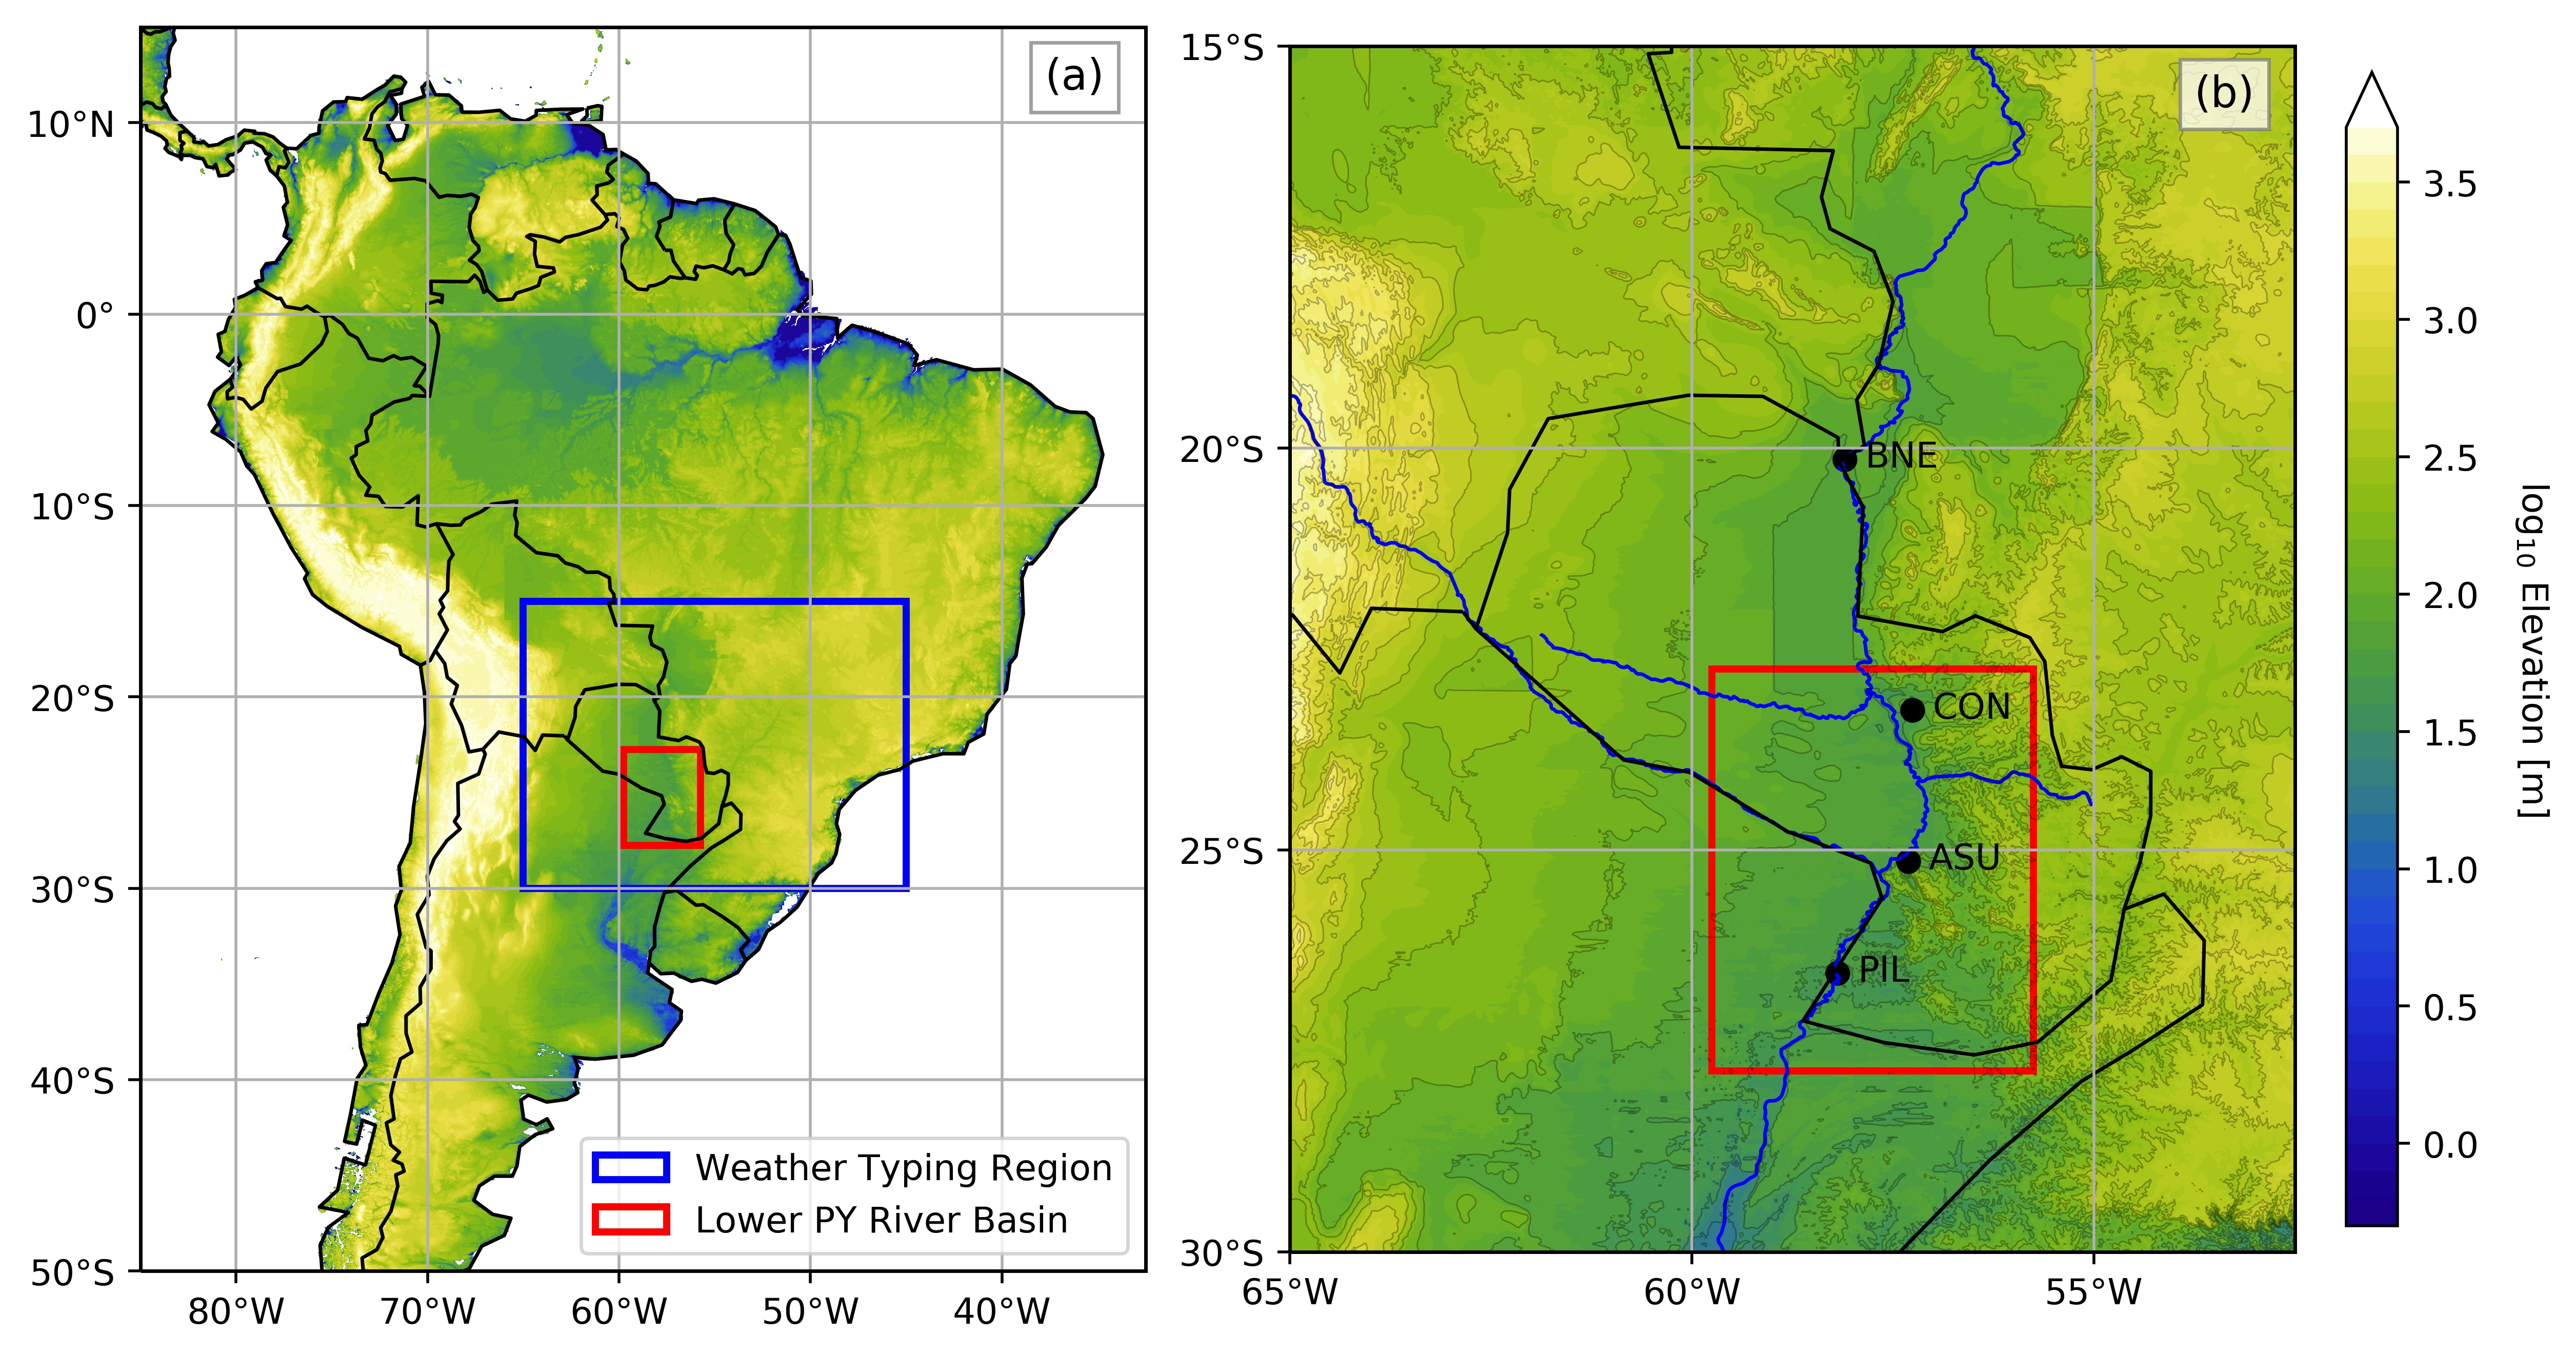
\includegraphics[width=6.5in]{study_area.jpg}
	\caption{
		Topographical map of the study area.
		Colors indicate $\log_{10}$ of elevation, in \si{\meter}, from the Global Land One-Km Base Elevation project available at \texttt{http://iridl.ldeo.columbia.edu/SOURCES/.NOAA/.NGDC/.GLOBE/.topo/}.
		(a): all of South America.
		The domains of the ``Lower Paraguay River Basin'' and the domain used for weather typing are indicated in red and blue, respectively.
		(b): The Paraguay River.
		As for (a), the ``Lower Paraguay River Basin'' is denoted with a red box.
		Streamflows shown in \cref{fig:streamflow} were taken from the fours stations indicated.
		The Paraguay River and its tributaries, from the Natural Earth database (\texttt{www.naturalearthdata.com}), are also shown.
		Full station names are: Bah\'ia Negra (Bne); Concepci\'on (Conc); Asunci\'on (Asu); Pilar (Pil).
	}\label{fig:study-area}
\end{figure*}

\begin{figure*}
	\noindent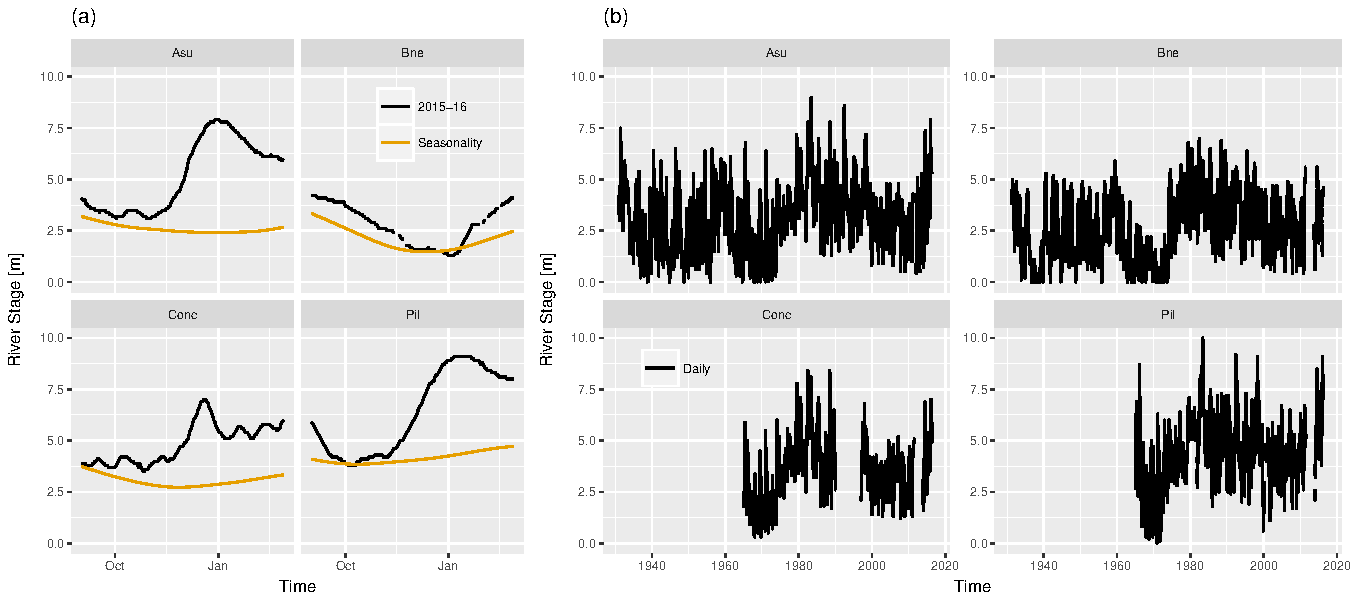
\includegraphics[width=6.5in]{Streamflow.pdf}
	\caption{
		River stage (height; in \si{\meter}) for the Paraguay River at four gauges along the Paraguay River.
		The station names are shortened versions of those shown in \cref{fig:study-area}.
		(a) Seasonality (orange) and time series of 2015-16 observations (black) at each stream gauge.
			The seasonality was fit using local polynomial regression as implemented in the \texttt{locfit} package in
			the \textbf{R} statistical programming environment \citep{Loader1999}.
		(b) Time series of daily stage measurements from 1929 to 2016 at each station.
	}\label{fig:streamflow}
\end{figure*}

\begin{figure*}	\noindent\includegraphics[width=6.5in]{lagged_rain.pdf}
	\caption{
		Composite anomalies associated with heavy rainfall (\nth{90} percentile exceedance of area-averaged rainfall in the Lower Paraguay River Basin).
		Lagged composites are shown, by column, for $t = $ \SIlist{-2;-1;0;1}{\day} relative to the date of heavy rainfall.
		Top row (a-d) shows composite streamfunction anomalies at \SIlist{850}{\hecto\pascal}.
		Bottom row (e-h) shows composite rainfall anomalies, in units of \si{\milli\meter\per\day}.
	}\label{fig:lagged-rain}
\end{figure*}

\begin{figure*}
	\noindent\includegraphics[width=6.5in]{eof_loadings.pdf}
	\caption{
		Loadings of the four leading \glspl{eof} of daily NDJF \SI{850}{\hecto\pascal} streamfunction over the weather typing region shown in \cref{fig:study-area}.
		Parentheses indicate percentage of total variance explained by each EOF.
	}\label{fig:eof-loading}
\end{figure*}

\begin{figure*}
	\noindent\includegraphics[width=6.5in,height=9in,keepaspectratio=true]{wt_composite.pdf}
	\caption{
		Composite anomalies associated with each weather typ.
		Top row (a-f) shows streamfunction anomalies at \SIlist{850}{\hecto\pascal}.
		Bottom row (g-l) shows rainfall anomalies, in units of \si{\milli\meter\per\day}. 
		The relative frequency of occurrence of each weather type (in days) is presented on the top of each column.
	}
	\label{fig:wt-composite}
\end{figure*}

\begin{figure*}
	\noindent\includegraphics[width=6.5in]{rain_wt_201516.pdf}
	\caption{
		Time series of area-averaged rainfall in the Lower Paraguay River Basin (\cref{fig:study-area}) for each day of NDJF  2015-16.
		Lines indicate the raimfall value, in units of \si{\milli\meter\per\day}.
        The weather type corresponding to each day is indicated in an adjacent text label.
		Dashed lines blue indicate (from bottom to top) the climatological 50th, \nth{90}, and 99th percentiles of NDJF area-averaged rain over the Lower Paraguay River basin.
	}\label{fig:rain-wt}
\end{figure*}

\begin{figure*}
	\noindent\includegraphics[width=6.5in]{anomalies_ndjf1516.pdf}
	\caption{
		Monthly composite anomalies observed during NDJF 2015-16.
		Top row (a-d) shows streamfunction anomalies at \SI{850}{\hecto\pascal}.
		Bottom row (e-h) shows rainfall anomalies, in units of \si{\milli\meter\per\day}.
	}\label{fig:anomalies}
\end{figure*}

\begin{figure*}
	\noindent\includegraphics[width=3.5in]{seasonal_forecast.pdf}
	\caption{
		Seasonal model forecast for probability of exceedance of \nth{90} percentile of DJF rainfall.
		Color indicates the forecast probability of exceeding the \nth{90} percentile of climatological rainfall during DJF 2015-16 -- this is presented as the odds ratio as defined in \cref{eq:odds-ratio}.
		A value greater than 1 indicates that the model forecast greater-than-average odds of rainfall exceeding the \nth{90} percentile.
		Grid cells which observed an exceedance of the \nth{90} percentile of DJF rainfall are outlined in black.
	}\label{fig:seas-prob-fcst}
\end{figure*}

\begin{figure*}
	\noindent\includegraphics[width=6.5in]{chiclet.pdf}
	\caption{
		Chiclet diagram \citep{Carbin:2016fx} of ensemble-mean precipitation anomaly forecasts over the Lower Paraguay River Basin (see \cref{fig:study-area}) from ECMWF S2S forecast data, as a function of the forecast target date (horizontal axis) and lead time (vertical axis).
		Time series of CPC daily mean precipitation over the same area is plotted with $y$-axis inverted; horizontal black line denotes NDJF climatology.
	}\label{fig:chiclet}
\end{figure*}

\begin{figure*}
	\noindent\includegraphics[width=6.4in]{mos_forecasts.pdf}
	\caption{
		MOS-adjusted S2S model forecasts and skill scores for the methods indicated in \cref{tab:mos-methods}.
		Top row (a-e) shows the heavy rainfall forecast for 1-7 December 2015 as the odds ratio defined in \cref{eq:odds-ratio} over the target domain.
		A value greater than 1 indicates that the model forecast greater-than-average odds of rainfall exceeding the \nth{90} percentile.
        Second row (f-j) shows the Ignorance score defined in \cref{eq:ignorance}, with zero indicating a perfect forecast.
		Bottom row (k-o) shows the 2AFC skill score for each grid cell; a value greater than 50 indicates that the model outperforms climatology.
		Columns separate different \gls{mos} models except ``Raw'', which indicates the uncorrected S2S model output.
		For all rows the grid cells which experienced a \nth{90} percentile exceedance for 1-7 December 2015 are outlined in black.
	}\label{fig:subs-prob-fcst}
\end{figure*}

\begin{figure*}
	\noindent\includegraphics[width=6.4in]{wt_mjo_enso.pdf}
	\caption{
		Anomalous probability of occurrence of each weather type concurrent with observance of each \gls{mjo}  phase.
		MJO phases are considered here only when the amplitude $\qty(\sqrt{\text{RMM1}^2 + \text{RMM2}^2})$ is greater than 1.
		When amplitude $< 1$, the phase is defined as neutral (0).
		Plots are shown separately for El Ni\~no, La Ni\~na, and neutral \gls{enso} months, defined by the NINO 3.4 index having a value above 1 or below -1.
		Only values which are significant at $p<0.10$, calculated using a bootstrap with 3000 samples, are shown.
	}\label{fig:wt-mjo-enso}
\end{figure*}

\begin{figure*}
	\noindent\includegraphics[width=6.4in]{ChacoNoChacojet.pdf}
	\caption{
		Schematics of low-level jet events (red arrows) during austral summer and El Ni\~no years.
		Most jet events are of the ``Chaco'' type, particularly when SST anomalies in the central southern Atlantic Ocean (a, see green box) are weak.
		When a dipolar SST anomaly occurs in the central southern Atlantic with the warmer pole equatorward, the meridional temperature gradient and sea-land temperature contrasts establish an anti-cyclonic circulation (dot-dashed line) conducive to increased occurrence of No-Chaco jet events (b).
		Other SST anomaly configurations tend to be present outside the green box (not shown).
		Winds in panels are typical for each case (at \SI{850}{\hecto\pascal}).
		Reference wind vector in \si{\meter\per\second}.
	}\label{fig:chaco-nochaco}
\end{figure*}

\begin{figure*}
	\noindent\includegraphics[width=6.4in]{sst_anomalies.pdf}
	\caption{
		Composite sea surface temperature (SST) anomalies from \citet{Reynolds:2002iy}.
		(a): The Pearson correlation of each SST grid cell with the time series of average zonal wind over the region indicated by the blue box.
		(b): Sea surface temperature (SST) anomalies during December 2015.
		Both panels show the Central Southern Atlantic with a black box; this is the same region as shown in \cref{fig:chaco-nochaco}.
	}\label{fig:wt4-months}
\end{figure*}

\end{document}
